\input{preambuloSimple.tex}
\title{	
	\normalfont \normalsize 
	\textsc{{\bf Ingeniería de Servidores (2016-2017)} \\ Grado en Ingeniería Informática \\ Universidad de Granada} \\ [25pt] % Your university, school and/or department name(s)
	\horrule{0.5pt} \\[0.4cm] % Thin top horizontal rule
	\huge Práctica 5. Ajuste del sistema. \\ % The assignment title
	\horrule{2pt} \\[0.5cm] % Thick bottom horizontal rule
}

\author{Manuel Jiménez Molina} % Nombre y apellidos

\date{\normalsize\today} % Incluye la fecha actual

%----------------------------------------------------------------------------------------
% DOCUMENTO
%----------------------------------------------------------------------------------------

\begin{document}
	
	\maketitle % Muestra el Título
	
	\newpage %inserta un salto de página
	
	\tableofcontents % para generar el índice de contenidos
	
	\listoffigures
	
	\listoftables
	
	\newpage
	
	%NOTA: en caso de problema al compilar, compruebe que tiene el paquete: texlive-babel-spanish.noarch  \\
	
	
	
	
	\newpage
	
	%----------------------------------------------------------------------------------------
	%	Cuestión 1
	%----------------------------------------------------------------------------------------
	
	\section{Al modificar los valores del kernel de este modo, no logramos que persistan después de reiniciar la máquina. ¿Qué archivo hay que editar para que los cambios sean permanentes?}
	
	El comando sysctl configura los parámetros del kernel en tiempo de ejecución. Con la opción -p carga en sysctl configuración de un archivo especificado o por defecto /etc/sysctl.conf\cite{ejercicio1-1}.\\
	Para que los cambios sean persistentes en el kernel tenemos que modificar el archivo /etc/sysctl.conf para que los cambios se carguen en cada reinicio\cite{ejercicio1-2}. Este archivo contiene valores de sysctl (valores del kernel) que pueden ser leídos por sysctl, el cual los configura para el kernel\cite{ejercicio1-3}.\\
	
	
	Cambiaremos la variable "shmmni" la cual establece el número máximo de segmentos de memoria compartida del sistema\cite{ejercicio1-4}. El valor actual de esta variable es:
	\begin{itemize}
		\item Vista desde el sistema de archivos /proc/sys/kernel.
			 \begin{figure}[H] 
			 	\centering
			 	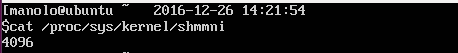
\includegraphics[scale=0.7]{ejercicio1-1.png} 
			 	\label{figura1} 
			 	\caption{Valor de variable kernel shmmni desde /proc/sys}
			 \end{figure}
		\item Vista usando la orden sysctl.
			\begin{figure}[H] 
				\centering
				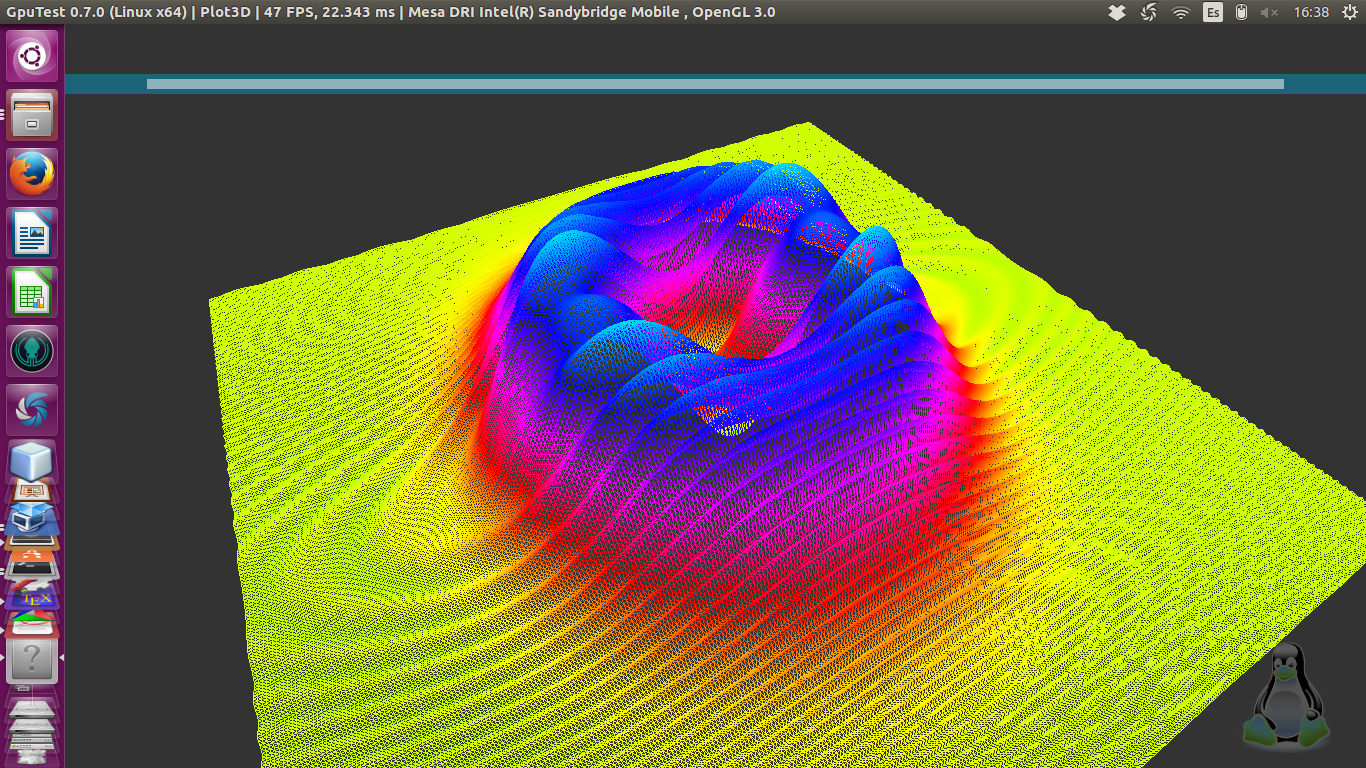
\includegraphics[scale=0.7]{ejercicio1-2.png} 
				\label{figura2} 
				\caption{Valor de variable kernel shmmni con comando sysctl}
			\end{figure}
	\end{itemize}
	
	Vamos a comprobar cada caso para ver si los cambios serán persistentes o no:
	\begin{itemize}
		\item Los cambios usando solo sysctl no son persistentes:
			\begin{itemize}
				\item Cambiamos shmmni con sysctl.
					\begin{figure}[H] 
						\centering
						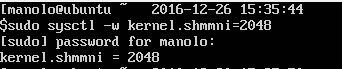
\includegraphics[scale=0.7]{ejercicio1-3.png} 
						\label{figura3} 
						\caption{Cambiar parámetro shmmni con sysctl}
					\end{figure}
				\item Comprobamos que se ha cambiado correctamente.
					\begin{figure}[H] 
						\centering
						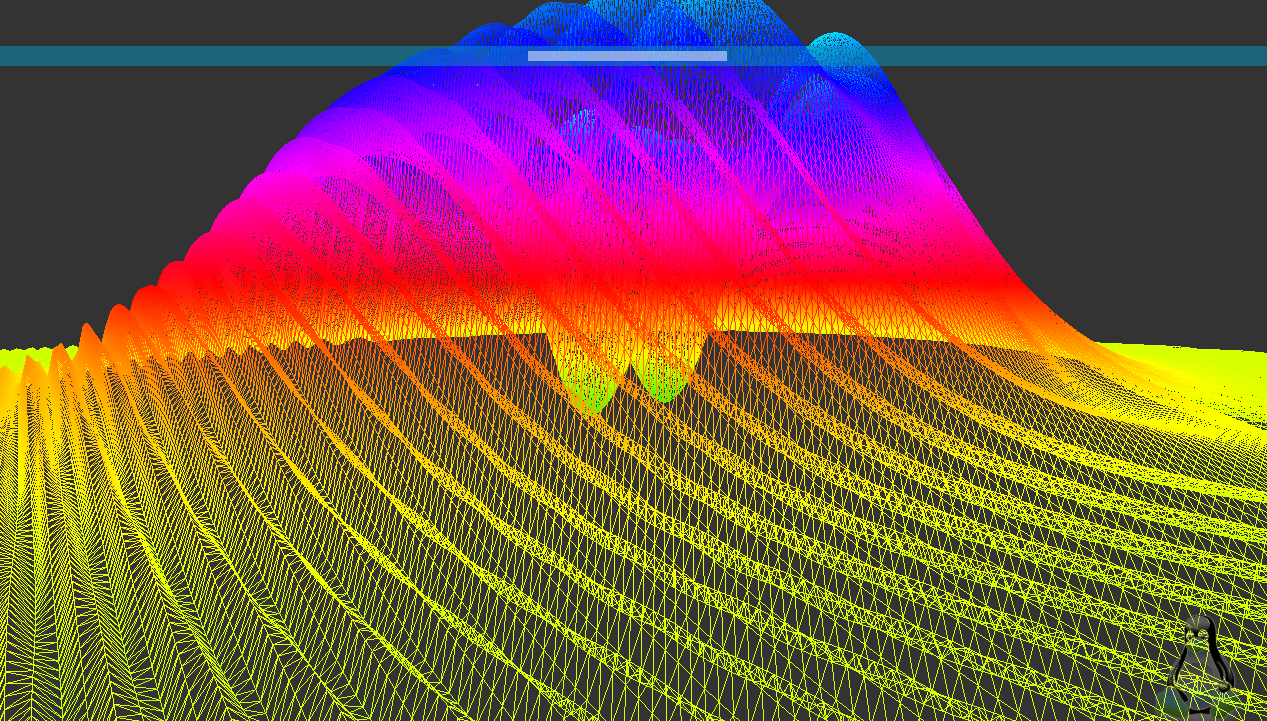
\includegraphics[scale=0.7]{ejercicio1-4.png} 
						\label{figura4} 
						\caption{Comprobar parámetro shmmni con sysctl}
					\end{figure}
				\item Reiniciamos y comprobamos su valor.
					\begin{figure}[H] 
						\centering
						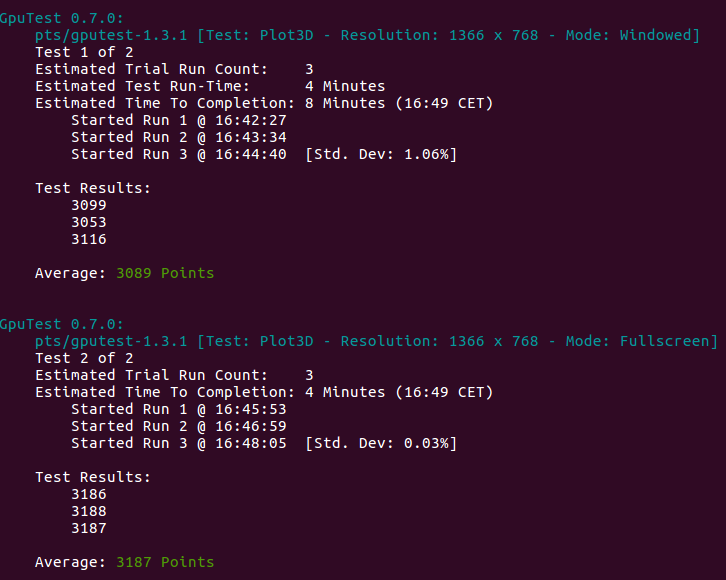
\includegraphics[scale=0.7]{ejercicio1-5.png} 
						\label{figura5} 
						\caption{Comprobar parámetro shmmni con sysctl tras reiniciar}
					\end{figure}
			\end{itemize}
		\item Los cambios modificando el archivo /etc/sysctl.conf son persistentes tras un reinicio:
			\begin{itemize}
				\item Cambiamos parámetro shmmni modificando el archivo /etc/sysctl.conf.
					\begin{figure}[H] 
						\centering
						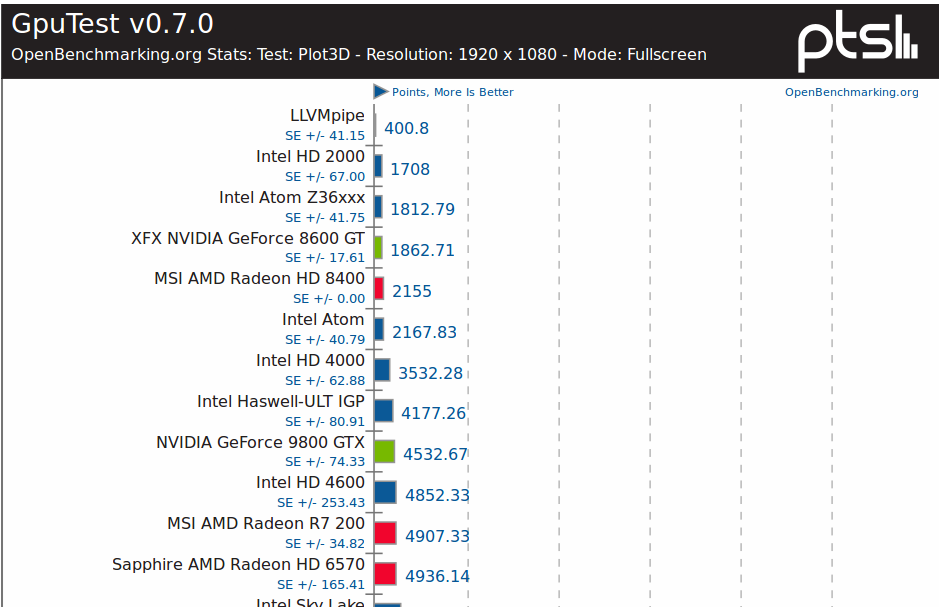
\includegraphics[scale=0.7]{ejercicio1-6.png} 
						\label{figura6} 
						\caption{Cambiar parámetro shmmni en /etc/sysctl.conf}
					\end{figure}
				\item Usamos sysctl -p para que los cambios tenga efecto y cargue el archivo correctamente.
					\begin{figure}[H] 
						\centering
						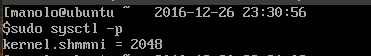
\includegraphics[scale=0.7]{ejercicio1-7.png} 
						\label{figura7} 
						\caption{Cargar configuración por defecto con sysctl}
					\end{figure}
				\item Comprobamos que el valor está cambiado antes del reinicio.
					\begin{figure}[H] 
						\centering
						
\includegraphics[scale=0.7]{ejercicio1-8.png} 
						\label{figura8} 
						\caption{Comprobar parámetro shmmni con sysctl}
					\end{figure}
				\item Reiniciamos y comprobamos que el valor ahora sí sigue cambiado:
					\begin{figure}[H] 
						\centering
						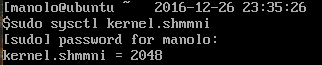
\includegraphics[scale=0.7]{ejercicio1-9.png} 
						\label{figura9} 
						\caption{Comprobar parámetro shmmni con sysctl tras reiniciar}
					\end{figure}
			\end{itemize}
	\end{itemize}
	
	
	%----------------------------------------------------------------------------------------
	%	Cuestión 2
	%----------------------------------------------------------------------------------------
	
	\section{¿Con qué opción se muestran todos los parámetros modificables en tiempo de ejecución? Elija dos parámetros y explique, en dos líneas, qué función tienen.}
	
	Para ver todos los parámetros modificables actuales en tiempo de ejecución usamos la orden sysctl -a \cite{ejercicio1-1}. Como hay muchos parámetros los meteremos en un fichero llamado parametros.data .\\
	
	Metemos los parámetros en el archivo parametros.data.
		\begin{figure}[H] 
			\centering
			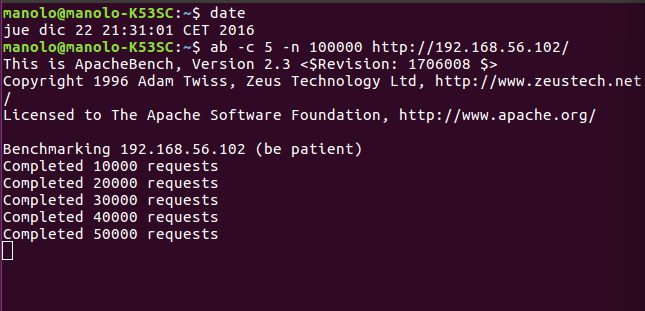
\includegraphics[scale=0.7]{ejercicio2-1.png} 
			\label{figura10} 
			\caption{Orden sysctl -a hacia archivo parametros.data}
		\end{figure}
	
	Miramos el contenido del archivo parametros.data.
	\begin{figure}[H] 
		\centering
		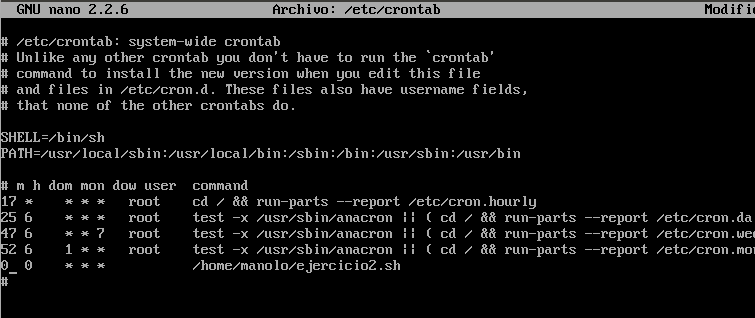
\includegraphics[scale=0.7]{ejercicio2-2.png} 
		\label{figura11} 
		\caption{Miramos dentro de parametros.data}
	\end{figure}
	
	Por ejemplo vamos a elegir dos parámetros \cite{ejercicio2-1}:
	\begin{itemize}
		\item \textbf{kernel.dmesg\_restrict}: Indica si los usuarios no privilegiados no pueden usar dmesg para ver los mensajes del buffer de registro del kernel. Cuando se establece a 0 no hay restricciones. Cuando se establece a 1, los usuarios deben tener CAP\_SYSLOG para usar dmesg.
		\item \textbf{kernel.hung\_task\_panic}: Controla el comportamiento del kernel cuando se detecta una tarea que se queda colgada (o bloqueada para siempre). Este archivo aparece si CONFIG\_DETECT\_HUNG\_TASK está habilitado.\\
		Con el valor 0, la operación continuaría (comportamiento predeterminado).\\
		Con valor 1, entraría en pánico de inmediato.
	\end{itemize}
	
	%----------------------------------------------------------------------------------------
	%	Cuestión 3
	%----------------------------------------------------------------------------------------
	
	\section{a) Realice una copia de seguridad del registro y restáurela, ilustre el proceso con capturas. b) Abra una ventana mostrando el editor del registro.}
	
	
	\subsection{a) Realice una copia de seguridad del registro y restáurela, ilustre el proceso con capturas.}
	
	Podemos encontrar documentación oficial de Microsoft para realizar una copia de seguridad del registro y restaurarla.\\
	
	Primero crearemos una copia de seguridad del registro para posteriormente restaurarla.
	\begin{itemize}
		\item Pulsamos inicio y escribimos regedit.
			\begin{figure}[H] 
				\centering
				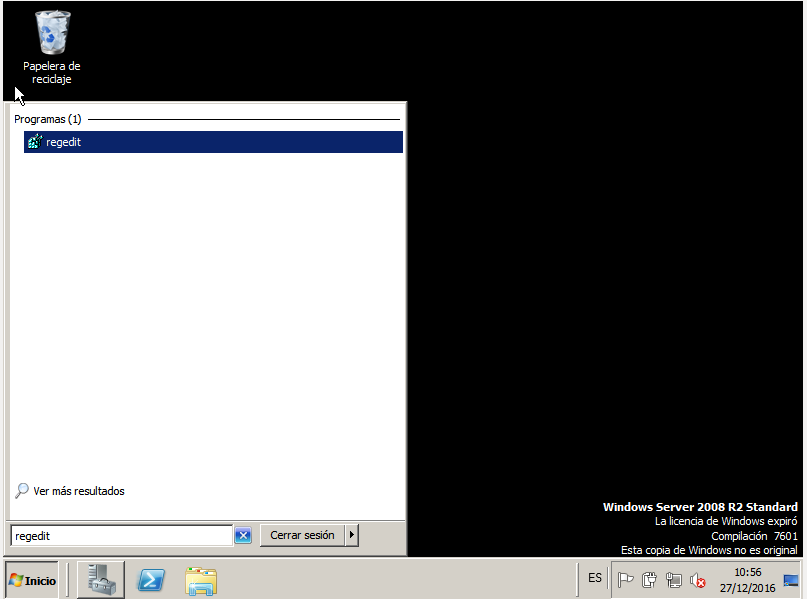
\includegraphics[scale=0.5]{ejercicio3-1.png} 
				\label{figura12} 
				\caption{Buscar en inicio regedit}
			\end{figure}
		\item Abrimos el registro pulsando en regedit. Nos aparecerán una lista de directorios que contendrán valores de configuración del sistema.
			\begin{figure}[H] 
				\centering
				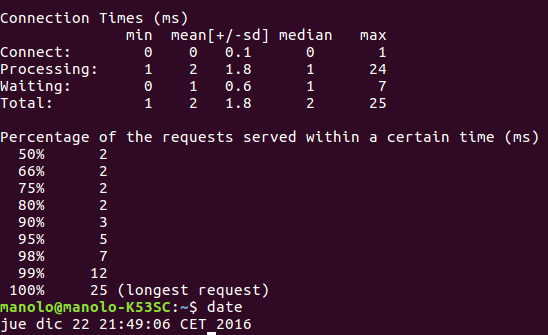
\includegraphics[scale=0.5]{ejercicio3-2.png} 
				\label{figura13} 
				\caption{Abrir registro en Windows}
			\end{figure}
		\item Hacemos click derecho sobre "Equipo" y le damos a exportar.
				\begin{figure}[H] 
					\centering
					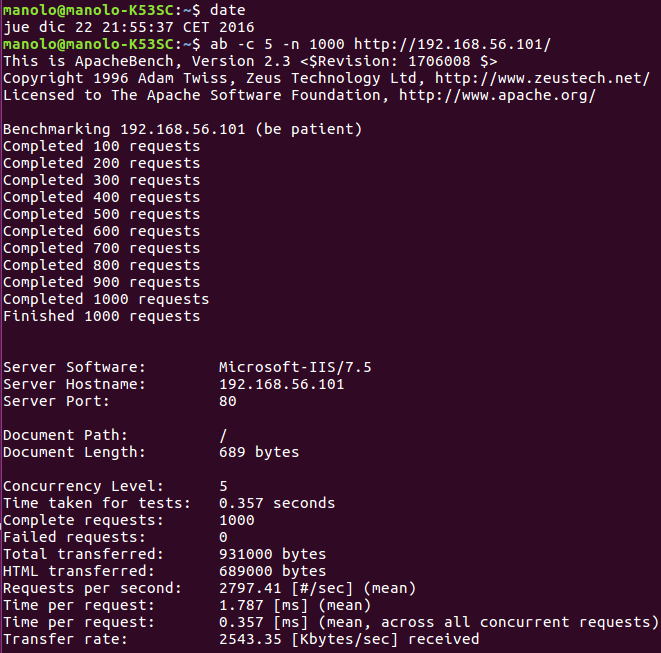
\includegraphics[scale=0.5]{ejercicio3-3.png} 
					\label{figura14} 
					\caption{Exportar registro}
				\end{figure}
		\item Elegimos directorio donde guardar registro y terminamos dándole a "Guardar".
			\begin{figure}[H] 
				\centering
				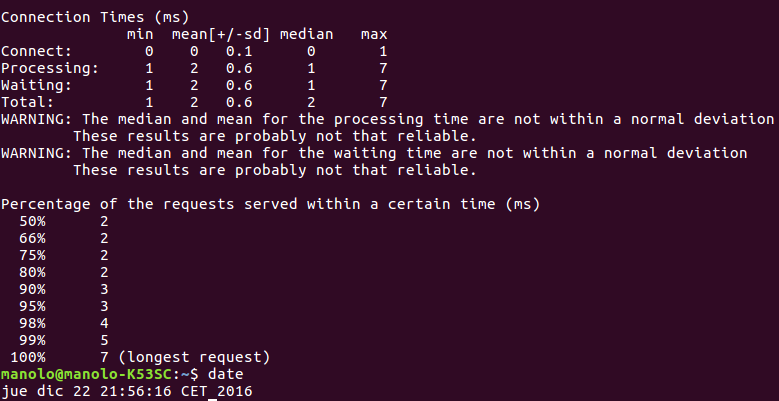
\includegraphics[scale=0.5]{ejercicio3-4.png} 
				\label{figura15} 
				\caption{Elegir directorio donde exportar registro y terminar}
			\end{figure}
		\item Comprobamos que ha sido guardada correctamente mirando el directorio con PowerShell.
			\begin{figure}[H] 
				\centering
				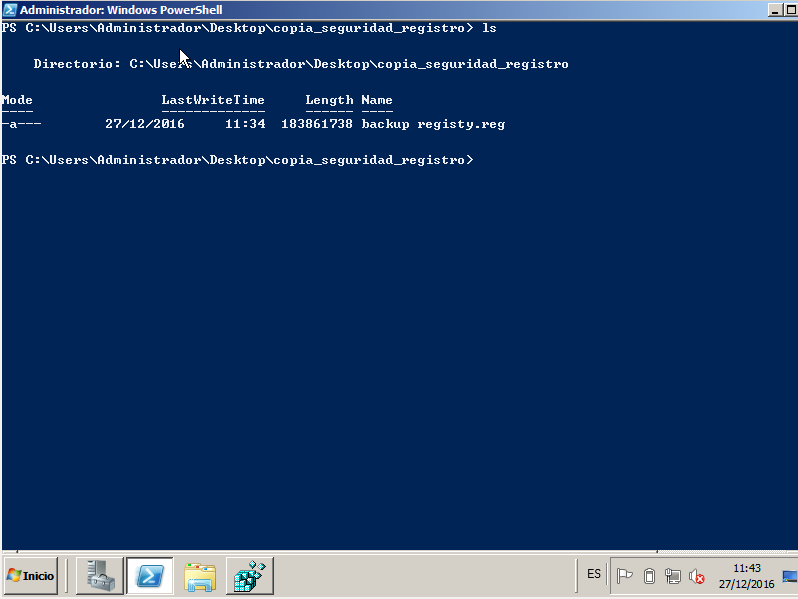
\includegraphics[scale=0.5]{ejercicio3-5.png} 
				\label{figura16} 
				\caption{Comprobar la copia del registro en el directorio con PowerShell}
			\end{figure}
	\end{itemize}
	
	Ya tenemos la copia de seguridad del registro guardada en una carpeta llamada copia\_seguridad\_registro.\\
	
	Procedemos a restaurar la copia que hemos realizado. Para ello se hará lo siguiente:
	\begin{itemize}
		\item Volvemos a escribir regedit en inicio para abrir el registro.
		\item Una vez abierto el registro, nos vamos a su menú desplegable y elegimos "Archivo" > "Importar".
			\begin{figure}[H] 
				\centering
				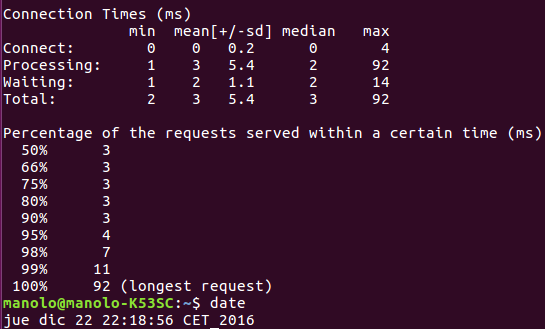
\includegraphics[scale=0.5]{ejercicio3-6.png} 
				\label{figura17} 
				\caption{Importar registro}
			\end{figure}
		\item Seleccionamos la carpeta que contenía la copia de seguridad del registro.
			\begin{figure}[H] 
				\centering
				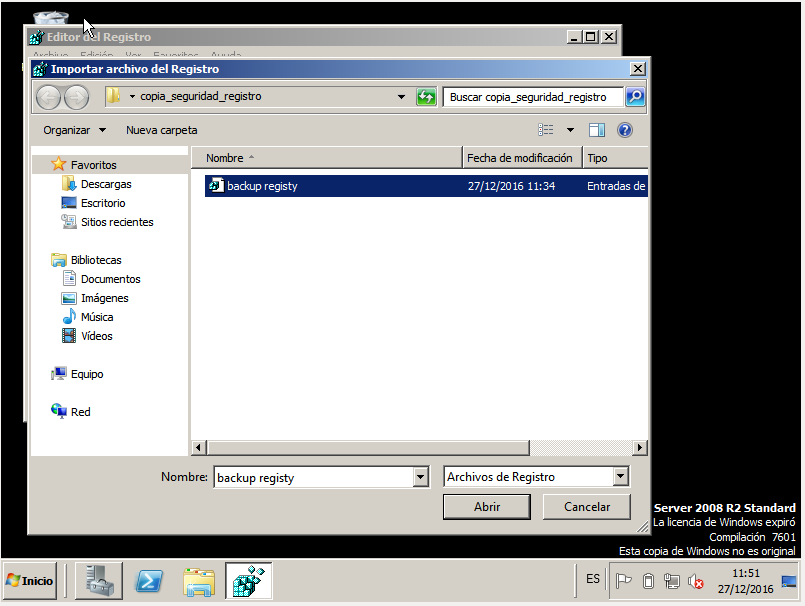
\includegraphics[scale=0.5]{ejercicio3-7.png} 
				\label{figura18} 
				\caption{Seleccionar archivo para importar el registro}
			\end{figure}
		\item Acaba el proceso de restauración del registro.
			\begin{figure}[H] 
				\centering
				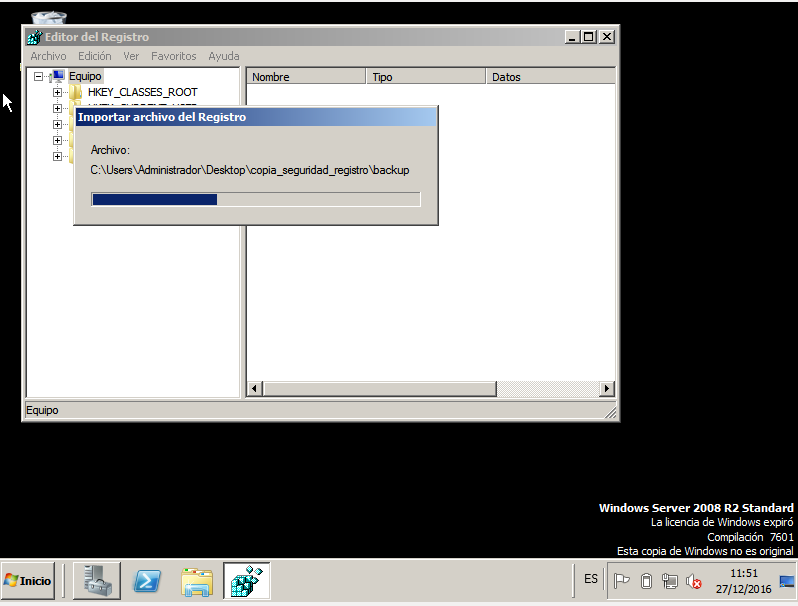
\includegraphics[scale=0.5]{ejercicio3-8.png} 
				\label{figura19} 
				\caption{Finalizando restauración del registro}
			\end{figure}
		
	\end{itemize}
	\subsection{b) Abra una ventana mostrando el editor del registro.}
	
	Encontramos una referencia de Windows de información de registro para usuarios avanzados\cite{ejercicio3-2}. Podemos abrir el editor del registro abriendo una consola del sistema (cmd) y escribiendo regedit.
	
	\begin{figure}[H] 
		\centering
		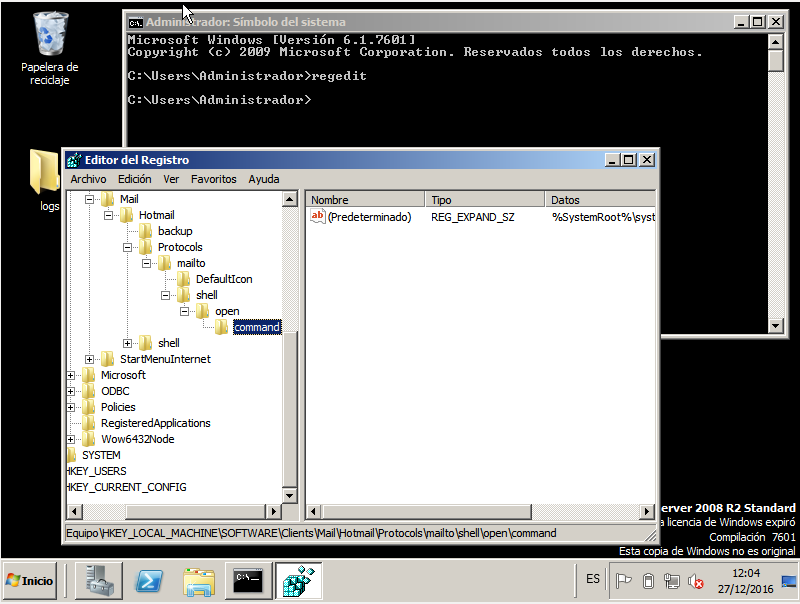
\includegraphics[scale=0.5]{ejercicio3-9.png} 
		\label{figura20} 
		\caption{Ventana de editor del registro}
	\end{figure}
	
	%	Cuestión 4
	%-----------------------------------------------
	\section{Enumere qué elementos se pueden configurar en Apache y en IIS para que Moodle funcione mejor.}
	
	Viendo la referencia de la práctica\cite{ejercicio4-1}, tenemos una serie de elementos a configurar para mejorar cualquier servidor:
	
	\begin{itemize}
		\item Escalabilidad:
		\begin{itemize}
			\item Si es un sitio web grande, separar la web de la base de datos.
			\item Si es un sitio web pequeño, tener base de datos y web juntas.
			\item Conseguir balanceo de carga, para compartir el trabajo entre varios servidores web. Se deberían usar más de un servidor web, que consultan a una mismo base de datos y hacen referencia a un mismo área de archivos.
		\end{itemize}
		\item Configuración hardware:
		\begin{itemize}
			\item Aumentar RAM del servidor web.
			\item Aumentar memoria principal (para reducir cambio a disco y permitir a tu servidor soportar y gestionar más usuarios).
			\item Mejorar el rendimiento obteniendo la mejor capacidad de procesador que puedas (dual o dual core por ejemplo).
			\item Tener una BIOS moderna para permitir hyperthreading.
			\item Usar discos duros SCSI mejor que SATA. Esto se debe a que SATA incrementa la utilización de CPU mientras que SCSI tiene procesadores propios integrados que son usados al tener múltiples dispositivos.
			\item Comprar discos duros con un tiempo de búsqueda bajo para aumentar de acceso a informes de Moodle.
			\item Establece un tamaño de archivos de intercambio correctamente. Recomendado ponerlo a 4 x RAM física.
			\item Usar un sistema de disco RAID.
			\item Usar gigabit ethernet para mejorar latencia y rendimiento.
			\item Comprobar configuración de la tarjeta de red. Puede obtener mejor rendimiento aumentando el uso de buffers en los descriptores de transimisión y recepción.
		\end{itemize}
		\item Sistema operativo:
		\begin{itemize}
			\item Usar Linux (recomendado), Windows o Mac OS X para el sistema operativo del servidor. Los sistemas operativos Unix requieren menos memoria que Mac OS X o Windows Server para realizar las mismas tareas. Además Linux no necesita licencia, pero puede ser difícil de aprender.
			\item Comprobar instrucciones específicas del fabricante para optimizar.
		\end{itemize}
		\item Rendimiento servidor web:
		\begin{itemize}
			\item Instalar Firefox y la extensión firebug para saber el tiempo de carga de cada componente de la página.
		\end{itemize}
		\item Rendimiento PHP:
		\begin{itemize}
			\item Usar PHP accelerator para facilitar la carga de CPU, como APC, PHPA, WinCache.
			\item Mejoras en rendimiento de lecturas/escrituras alojando las páginas PHP almacenadas en caché en un sistema de archivos TMPFS.
		\end{itemize}
	\end{itemize}
	
	\subsection{Elementos a configurar en Apache para que Moodle funcione mejor}
	
	Los elementos recomendados a cambiar en Apache para mejorar el funcionamiento de Moodle son los siguientes:
	
	\begin{itemize}
		\item Si usas Apache en servidor Windows, \textbf{utilizar compilación de Apache Lounge}, la cual informa de tener mejoras en rendimiento y estabilidad.
		\item Establecer directivas \textbf{MaxClients} correctamente. Debes usar esta fórmula:	
		\begin{center}
			\begin{math}			
				MaxClients = \dfrac{Memoria\ total\ disponible * 80\%}{Uso\ de\ memoria\ máximo\ de\ proceso\ Apache}	
			\end{math}
		\end{center}
		El uso de memoria de Apache para un proceso en normalmente 10MB, pero Moodle podría usar fácilmente hasta 100 MB por proceso, por lo que se divide la memoria disponible en MB por 100 para obtener una configuración adecuada para MaxClients.\\
		Si estableces MaxClients a mas de 256, tienes que establecer la directiva ServerLimit.
		\item \textbf{Reducir el número de módulos} que carga Apache en el archivo httpd.conf con el fin de reducir la memoria necesaria.
		\item Usar la \textbf{última versión de Apache}.
		\item Para sistemas Unix/Linux, podría reducir \textbf{MaxRequestPerChild} en httpd.conf hasta 20-30.
		\item Para un servidor muy cargado, puede desactivar \textbf{KeepAlive} (si sus páginas de Moodle no contienen enlaces a recursos o imágenes subidas) o bajando \textbf{KeepAliveTimeOut} entre 2 y 5. Cuanto más grande sea este valor, más procesos del servidor estarán esperando conexiones que seguramente inactivas. Para saber realmente el valor de KeepAliveTimeOut tendríamos que observar el tiempo que tardan los usuarios en descargar una página.
		\item Como alternativa a KeepAlive desactivado, podemos c\textbf{onfigurar un servidor proxy} para almacenar en caché archivos HTML con imágenes.
		\item Si no usas el archivo .htaccess, puedes establecer la variable \textbf{AllowOverride} a nada para evitar búsquedas de .htaccess. 
		\item Evitar negociación de contenido estableciendo \textbf{DirectoryIndex} correctamente.
		\item Si no estás desarrollando en el servidor, pon \textbf{ExtendedStatus Off} y deshabilita mod\_info y mod\_status.
		\item Deja \textbf{HostnameLookups Off} para reducir latencia DNS.
		\item Considerar reducir el valor de \textbf{TimeOut} entre 30-60 segundos.
		\item Configurar Apache para que cargue las páginas mucho más rápido \textbf{especificando que el navegador debe almacenar en caché elementos} como imágenes y reutilizarlos en la memoria local en vez de pedirlos cada vez que se solicita la página. Son 2 pasos:
			\begin{itemize}
				\item Instalar y habilitar \textbf{mod\_expires}.
				\item Agregar este código al archivo de configuración del servidor virtual dentro de la sección <directorio> para el directorio root (o con el archivo .htaccess si AllowOverrides está On):
					\begin{figure}[H] 
						\centering
						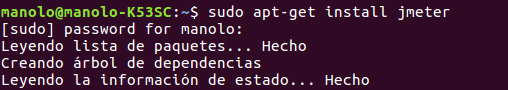
\includegraphics[scale=0.5]{ejercicio4-1.png} 
						\label{figura21} 
						\caption{Código para cargar páginas en Apache más rápido usando caché}
					\end{figure}
			\end{itemize}
		Con esto todo permanece en caché nos HTML y XML, que cambian dinámicamente. \\
		La \textbf{compresión} reduce los tiempos de respuesta reduciendo el tamaño de la respuesta HTTP. Para ello:
			\begin{itemize}
				\item Instalar y habilitar mod\_deflate.
				\item Agregar este código al archivo de configuración del servidor virtual dentro de la sección <directorio> para el directorio root (o con el archivo .htaccess si AllowOverrides está On): 
					\begin{figure}[H] 
						\centering
						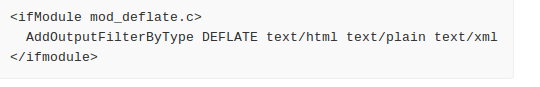
\includegraphics[scale=0.5]{ejercicio4-2.png} 
						\label{figura22} 
						\caption{Código para reducir tamaño respuesta HTTP}
					\end{figure}
			\end{itemize}
	\end{itemize}
	
	\subsection{Elementos a configurar en IIS para que Moodle funcione mejor}
	
	Los elementos recomendados a cambiar en IIS para que Moodle funcione mejor son los siguientes:
	\begin{itemize}
		\item El equivalente a KeepAliveTimeout es \textbf{ListenBackLog} (localizado en HKLM/SYSTEM/CurrentControlSet/Services/Inetinfo/Parameters). Establecer entre 2 y 5.
		\item Ajustar \textbf{MemCacheSize} a la cantidad de memoria (Mb) que ISS usará para archivos en caché.
		\item Cambiar el valor de \textbf{MaxCachedFileSize} para establecer el tamaño máximo de un archivo que está almacenado en caché en la caché de archivos en bytes.
		\item Crear un nuevo DWORD llamado \textbf{ObjectCacheTTL} para cambiar la duración del tiempo (milisegundos) que los objetos de caché están en memoria.
	\end{itemize}
	
	%----------------------------------------------------------------------------------------
	%	Cuestión 5
	%----------------------------------------------------------------------------------------
	
	\section{Ajuste la compresión en el servidor y analice su comportamiento usando varios valores para el tamaño de archivo a partir del cual comprimir. Para comprobar que está comprimiendo puede usar el navegador o comandos como curl (see url) o lynx. Muestre capturas de pantalla de todo el proceso.}
	
	
	Los cuellos de botella suelen estar mayormente en la red. Tenemos que enviar 1MB a un cliente para que pueda ver el contenido de una web, pero si comprimimos ese contenido y se lo enviamos, dicho envío será menor.\\
	
	Vamos a hacer que ISS comprima las páginas web. Miramos en el enlace proporcionado en el guión de prácticas para ver una guía de IIS de Microsoft\cite{ejercicio5-1}. En esta guía nos centraremos en la optimización de rendimiento de IIS\cite{ejercicio5-2}.\\
	
	Para optimizar el rendimiento, Microsoft nos ofrece dos características:
	\begin{itemize}
		\item Compresión: Para comprimir HTTP para hacer más eficiente el uso de banda ancha y aumentar el rendimiento de sitios web y aplicaciones. Se puede configurar para contenido estático y dinámico.
		\item Almacenamiento en caché de la salida: Permite administrar las reglas de almacenamiento en caché de salida y controlar el almacenamiento de caché del contenido servido.
	\end{itemize}
	
	Nos centraremos en la compresión. Windows nos proporciona las siguientes opciones de compresión\cite{ejercicio5-3}:
	\begin{itemize}
		\item Solo archivos estáticos.
		\item Solo respuestas dinámicas de la aplicación.
		\item Tanto archivos estáticos como respuestas dinámicas de la aplicación.
	\end{itemize}
	
	La compresión dinámica puede afectar a los recursos de la CPU ya que IIS no almacena en caché las versiones comprimidas de la salida dinámica. \\
	En cambio, las respuestas estáticas comprimidas se pueden almacenar en caché sin degradar los recursos de la CPU.\\
	
	Los pasos para realizar la compresión son \cite{ejercicio5-4,ejercicio5-5,ejercicio5-6}:
	\begin{itemize}
		\item Configurar compresión:
			\begin{itemize}
				\item Abrimos el administrador de IIS.
					\begin{figure}[H] 
						\centering
						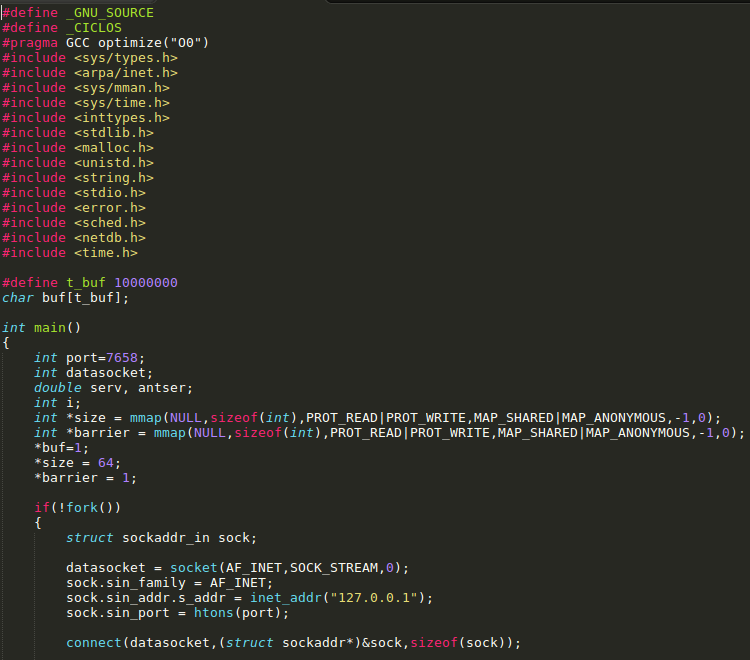
\includegraphics[scale=0.5]{ejercicio5-1.png} 
						\label{figura23} 
						\caption{Abrir administrador de IIS}
					\end{figure}
				\item Seleccionamos en el menú de la izquierda nuestro servidor y el su página principal (pantalla central) ponemos en el filtro de búsqueda la palabra "compresión".
					\begin{figure}[H] 
						\centering
						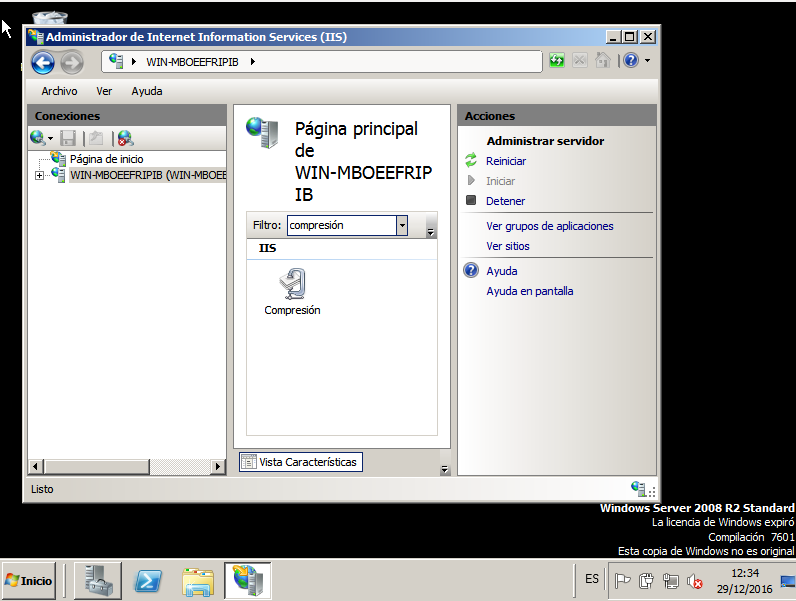
\includegraphics[scale=0.5]{ejercicio5-2.png} 
						\label{figura24} 
						\caption{Buscar compresión de la página principal de IIS}
					\end{figure}
				\item Seleccionamos compresión y comprobamos que esté activada la compresión estática y dejamos el tamaño de compresión a 2700 bytes.
					\begin{figure}[H] 
						\centering
						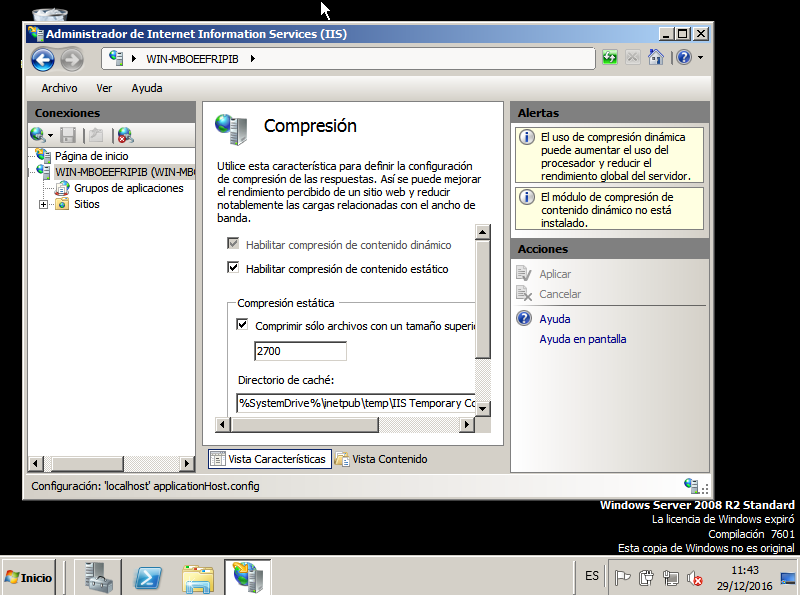
\includegraphics[scale=0.5]{ejercicio5-3.png} 
						\label{figura25} 
						\caption{Configurar compresión estática y tamaño de compresión}
					\end{figure}
			\end{itemize}
		\item Comprobación de la compresión. Para ello abriremos en la máquina anfitriona el navegador y miraremos el contenido de la cabecera de respuesta HTTP. La cabecera nos mostrará que existe una variable llamada "Accept-Encoding": "gzip,deflate" indicando que el contenido fue comprimido.
			\begin{figure}[H] 
				\centering
				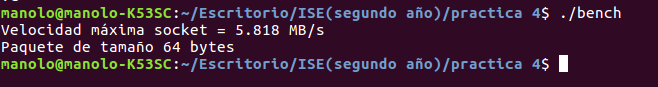
\includegraphics[scale=0.35]{ejercicio5-4.png} 
				\label{figura26} 
				\caption{Comprobación de compresión en cabecera http}
			\end{figure}
	\end{itemize}
	%----------------------------------------------------------------------------------------
	%	Cuestión 6
	%----------------------------------------------------------------------------------------
	
	\section{Usted parte de un SO con ciertos parámetros definidos en la instalación (Práctica 1), ya sabe instalar servicios (Práctica 2) y cómo monitorizarlos (Práctica 3) cuando los somete a cargas (Práctica 4). Al igual que ha visto cómo se puede mejorar un servidor web (Práctica 5 Sección 3.1), elija un servicio (el que usted quiera) y modifique un parámetro para mejorar su comportamiento. 6.b) Monitorice el servicio antes y después de la modificación del parámetro aplicando cargas al sistema (antes y después) mostrando los resultados de la monitorización.}
	
	
	Vamos a instalar el servidor web Nginx. Este servidor es una alternativa a Apache o también una complementación a este. Podría usarse junto a Apache, usando a Nginx como frontend y Apache como backend.\cite{ejercicio6-1,ejercicio6-2} \\
	Combinando ambos, tendremos una especie de dispositivo de descarga de red frente a los servidores Apache, consiguiendo que las conexiones lentas a Internet sean más rápidas y confiables por el lado del servidor, descargando conexiones keepalive (mensaje entre dispositivos para comprobar que la conexión entre ambos está operativa) de los servidores Apache. Con esto conseguimos un rendimiento de Apache como si estuviera a un "nivel local".\\
	
	Cabe destacar que Nginx protege a los servidores Apache de vulnerabilidades de picos en el tráfico o ataques de conexión lenta como por ejemplo Slowloris y slowquestprequest.\\
	
	Vamos a proceder a la instalación de Nginx en Ubuntu Server, la configuración de sus parámetros para mejoran su comportamiento, comprobado las mejoras mediante monitorización del servicio:
	
	
	\begin{itemize}
		\item \textbf{Instalamos Nginx}:
			\begin{itemize}
				\item 	sudo apt-get install nginx
			\end{itemize}
		\item \textbf{Configurar firewall para puerto 80:} 
			\begin{itemize}
				\item Comprobamos que el firewall (ufw) permite la conexión con el puerto 80. Sino, tenemos que habilitarla.
			\end{itemize}
		\item \textbf{Configurar red de Ubuntu Server}:
			\begin{itemize}
				\item Debemos configurar la red para establecer conexión entre la máquina anfitriona y la máquina virtual que tiene Nginx instalado.
			\end{itemize}
		\item \textbf{Comprobar que Nginx funciona correctamente}:
			\begin{itemize}
				\item Nos aseguramos que funciona Nginx. Probamos a conectarnos a la ip de la máquina virtual para ver su página de inicio.
				\begin{figure}[H] 
					\centering
					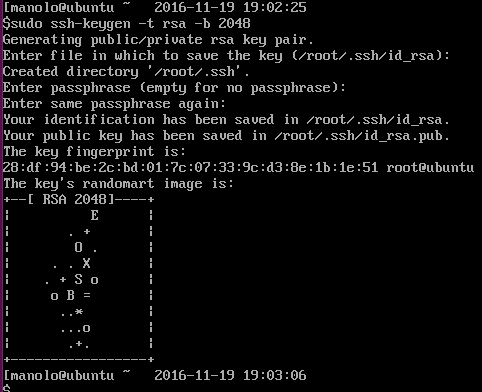
\includegraphics[scale=0.35]{ejercicio6-1.png} 
					\label{figura27} 
					\caption{Comprobar funcionamiento Nginx}
				\end{figure}
			\end{itemize}
		\item \textbf{Realizar test inicial}:
			\begin{itemize}
				\item Vamos a realizar un test de Nginx con Apache Benchmark (ab) desde la máquina anfitriona, monitorizando a la vez con top la máquina anfitriona.\\
				
				Ejecución de ab:
				\begin{figure}[H] 
					\centering
					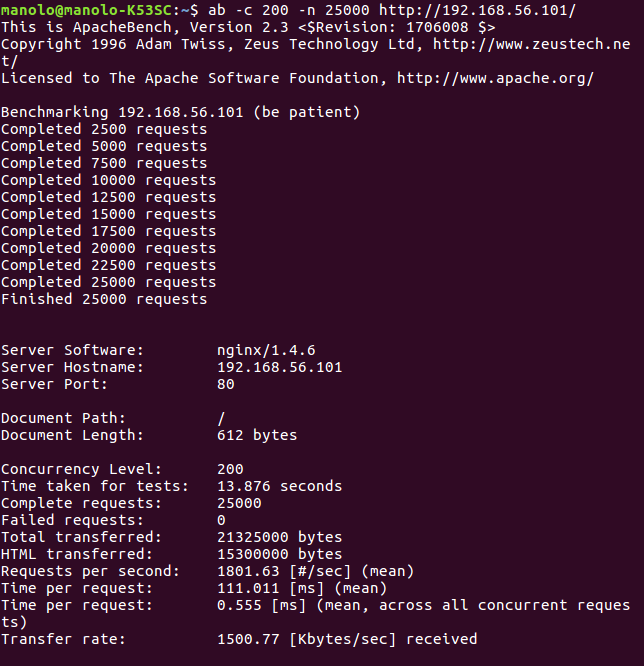
\includegraphics[scale=0.5]{ejercicio6-2.png} 
					\label{figura28} 
					\caption{Test inicial (foto 1). Nginx}
				\end{figure}
				\begin{figure}[H] 
					\centering
					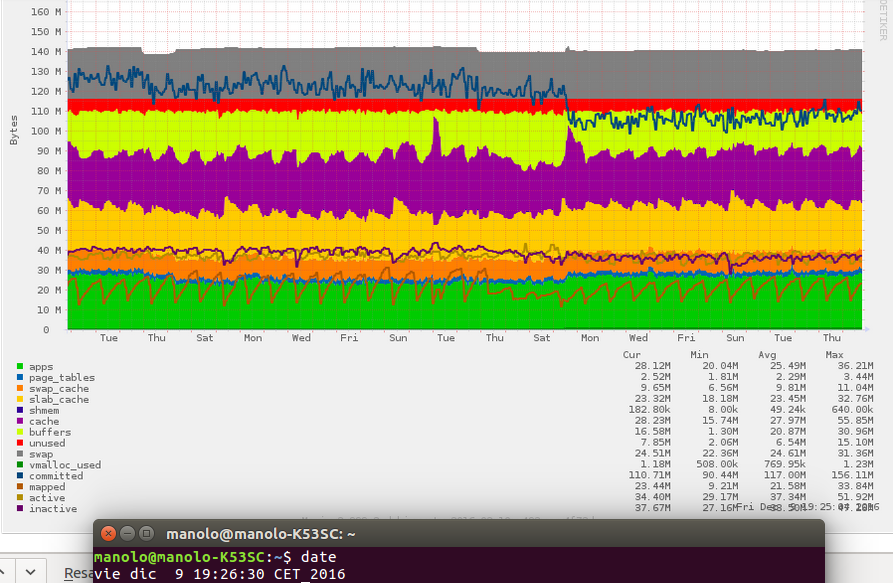
\includegraphics[scale=0.5]{ejercicio6-3.png} 
					\label{figura29} 
					\caption{Test inicial (foto 1). Nginx}
				\end{figure}
				
				Comprobación con ps:
				\begin{figure}[H] 
					\centering
					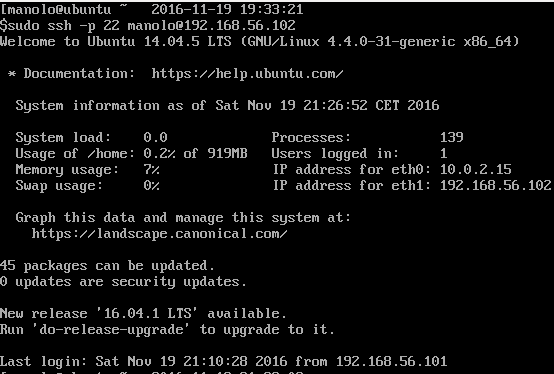
\includegraphics[scale=0.5]{ejercicio6-4.png} 
					\label{figura30} 
					\caption{Test inicial 1. Nginx}
				\end{figure} 
			Por la respuesta de ab, el tamaño de la página de inicio de Nginx es de 612 bytes. Para un nivel de concurrencia 200, para 25000 peticiones se ha tardado un total de 13.076 segundos.\\
			
			Por otra parte, viendo el comando top podemos ver como Nginx se llega a saturar un poco la cpu, alcanzando un pico de 39,2\%, teniendo valores entre 4,7\% y 39,2\%.
			\end{itemize}
		\item \textbf{Cambiando elementos para mejor rendimiento en Nginx}:
			\begin{itemize}
				\item Vamos a seguir unas recomendaciones de Nginx para mejorar el rendimiento de Nginx\cite{ejercicio6-3,ejercicio6-4,ejercicio6-5}. Dentro del archivo de configuración /etc/nginx/nginx.conf cambiaremos los siguientes parámetros:
				\begin{itemize}
					\item \textbf{worker\_processes}: Es el número de procesos de trabajos de Nginx. Lo establecemos a 8.
					\item \textbf{worker\_connections}: Número máximo de conexiones que cada proceso puede manejar simultáneamente. Lo establecemos dependiendo de la salida del comando ulimit -n (limitación del sistema). Será 1024.
					\item \textbf{keepalive\_timeout}: Tiempo que una conexión permanece abierta. Estará a 63 por defecto, pero lo establecemos a 3.
					\item \textbf{multi\_accept}: Se usa para que los 'workers' acepten todas las conexiones nuevas al mismo tiempo. Lo habilitamos.
				\end{itemize}
			
			\begin{figure}[H] 
				\centering
				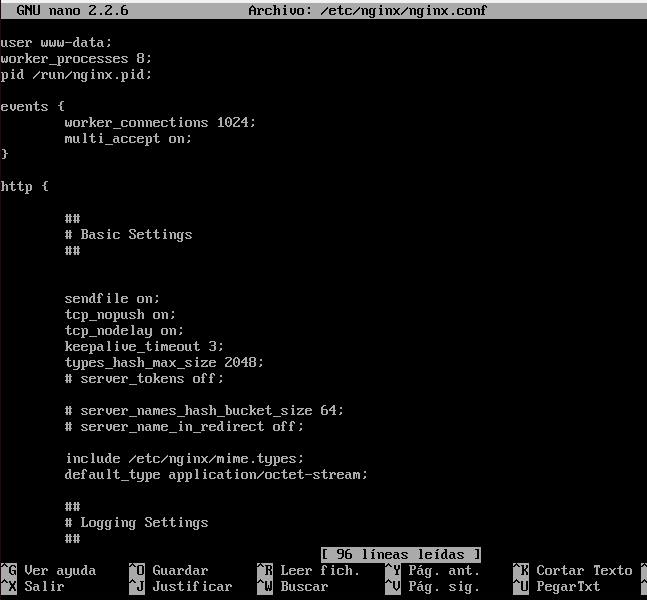
\includegraphics[scale=0.5]{ejercicio6-5.png} 
				\label{figura31} 
				\caption{Cambiando parámetros configuración Nginx}
			\end{figure} 	
			\end{itemize}
		\item \textbf{Restauramos el servicio Nginx para guardar los cambios}:
		\begin{itemize}
			\item sudo service nginx restart
		\end{itemize}
		\item \textbf{Comprobamos las mejoras de rendimiento}:
			\begin{itemize}
				\item Respecto a ab:
				\begin{figure}[H] 
					\centering
					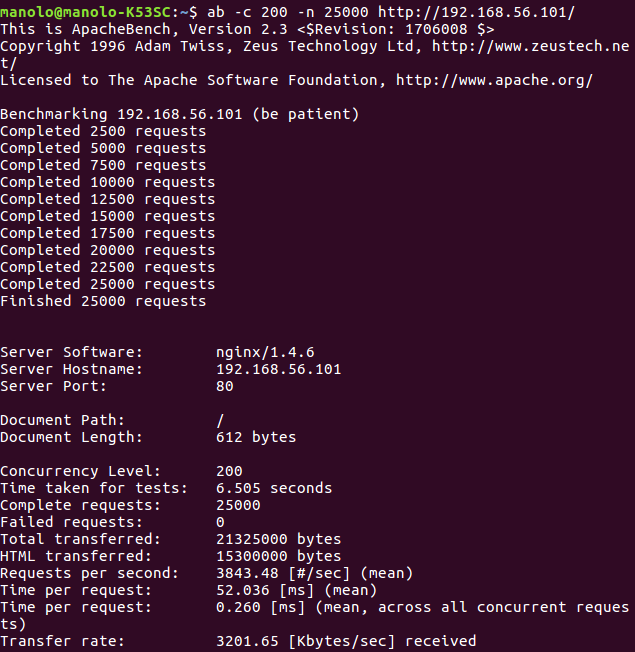
\includegraphics[scale=0.5]{ejercicio6-6.png} 
					\label{figura32} 
					\caption{Ab.Rendimiento Nginx tras cambiar parámetros (foto 1)}
				\end{figure}
				\begin{figure}[H] 
					\centering
					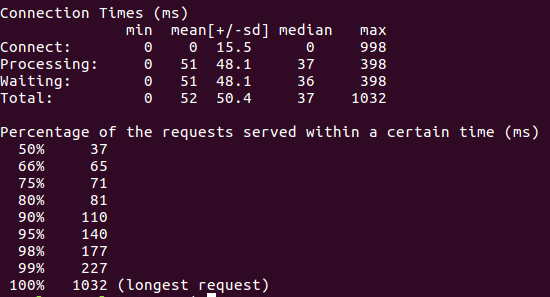
\includegraphics[scale=0.5]{ejercicio6-7.png} 
					\label{figura33} 
					\caption{Ab.Rendimiento Nginx tras cambiar parámetros (foto 2)}
				\end{figure}
			\end{itemize}
			\begin{itemize}
				\item Respecto a top:
				\begin{figure}[H] 
					\centering
					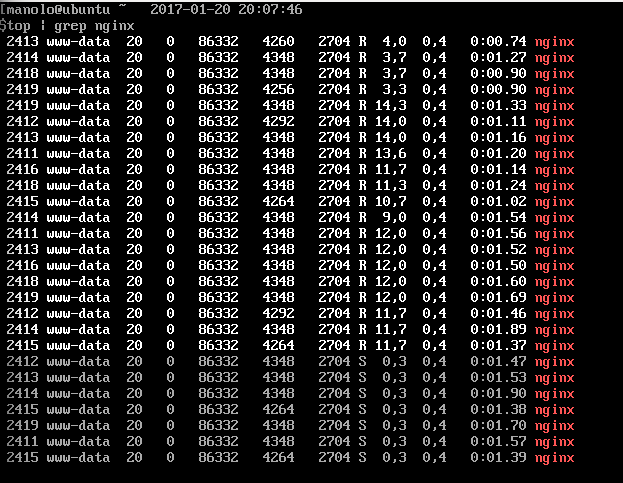
\includegraphics[scale=0.5]{ejercicio6-8.png} 
					\label{figura34} 
					\caption{Top. Rendimiento Nginx tras cambiar parámetros}
				\end{figure}
			\end{itemize}
		\item \textbf{Analizando nuevos resultados}: Hemos de decir que Nginx ya venía con valores por defecto que optimizan el servidor, como por ejemplo la compresión. 
			\begin{itemize}
				\item \textbf{Mejor tiempo de respuesta}. Con las mejoras realizadas, conseguimos un tiempo de 6.505 segundos frente a los 13.876 segundos sin las mejoras. Serían 7.371 segundos mejorados. 
				\item El tiempo por petición ha pasado de 0.555 ms a 0.260 ms. Esto supone una mejora de 0.295 ms por petición.
				\item \textbf{Existe una menor sobrecarga de CPU en el servidor}. Vemos como ahora no se llega si quiera al 20\%, mientras que antes se llegó incluso a 39\%.
				\item \textbf{Gracias a habilitar la variable multi\_accept, el rendimiento ha sido espectacular} (comprobé muchas veces y tras cambiarlo disminuyó hasta 6 segundos).
				
			\end{itemize}
	\end{itemize}
	

	Como conclusión decir que la mejora de rendimiento no me la esperaba, pero ha sido en mayor parte gracias a la variable multi\_accept. Las demás se notaban medio segundo o incluso menos. Se consigue tener un servidor menos sobrecargado y capaz de soportar más clientes y de responder de forma más eficiente.
	%----------------------------------------------------------------------------------------
	%	Cuestión opcional 1
	%----------------------------------------------------------------------------------------
	\section{Opcional 1: Realice lo mismo que en la cuestión 6 pero para otro servicio.}
	
	


	

%------------------------------------------------

\bibliography{citas} %archivo citas.bib que contiene las entradas 
\bibliographystyle{plain} % hay varias formas de citar

\end{document}
